Para el proceso de creación de la red 4G, se usó el \textit{software} srsRAN, una implementación de código abierto de una red de acceso radio (RAN) utilizando \textit{hardware} SDR.

Para ello, se siguieron los siguientes pasos:


\begin{enumerate}
\item Descarga de la última versión de \textbf{Ubuntu}, \textbf{22.04 LTS}.
\item Grabación de la ISO en un pincho a través de \textbf{UNetbootin} y posterior instalación de Linux en un ordenador sin sistema operativo (proporcionado por la empresa).
\item Instalación de los drivers de la \textit{Blade} siguiendo el manual de \textit{GitHub}:\\
 \url{https://github.com/Nuand/bladeRF/wiki/Getting-Started:-Linux}

\begin{lstlisting}
sudo add-apt-repository ppa:nuandllc/bladerf
sudo apt-get update
sudo apt-get install bladerf
\end{lstlisting}

\item Instalación de \textbf{srsran} siguiendo el manual de GitHub y las librerías \textbf{boost} y \textbf{libboost}:\\
\url{https://docs.srsran.com/projects/4g/en/latest/general/source/1_installation.html}\\
\url{https://docs.srsran.com/projects/4g/en/latest/getting_started.html}

\begin{lstlisting}
git clone https://github.com/srsRAN/srsRAN_4G.git
cd srsRAN_4G
mkdir build
cd build
cmake ../
make
make test
sudo make install
srsran_4g_install_configs.sh user
\end{lstlisting}

\item Modificación de los archivos de configuración que se encuentran en la ruta \textit{root/.config/srsran/}:
\begin{itemize}
	\item epc.conf: contiene la configuración específica de un controlador de paquetes Evolved Packet Core (EPC) en una arquitectura de red LTE 
	\item enb.conf: cotiene la configuración específica de un nodo de banda base (eNodeB).
	\item user_db.csv: que contiene una base de datos de usuarios en formato tabular.
\end{itemize}

En el archivo \textbf{enb.conf} se cambiaron los valores de \textbf{MCC} y \textbf{MNC} que están disponibles en las hojas de datos de las SIMs (y en la propia tarjeta SIM), y se establecieron sus valores correspondientes (\textbf{901-70}) para que correspondan con el IMSI. También se modificó el valor de la frecuencia central. cambiando el valor de \textbf{dl_earfcn}, para ello se utilizó \cite{earn}, estableciéndolo este valor 3050, lo que corresponde a un valor de frecuencia central \textit{downlink} de 2650.  Por último, se estableció el ancho de banda en 5MHz cambiando el valor de \textbf{n_prb} a \textbf{25}. Para mejorar el alcance de la red, se aumentó la ganancia de transmisor, cambiando el valor de \textbf{tx_gain} a 90.

En el archivo \textbf{epc.conf} se modificaron los valores de \textbf{MCC} y \textbf{MNC} (igual que en el caso anterior) y se añadieron los nombres de la red con:
\begin{lstlisting}
    full_net_name= NOMBRE
    short_net_name= NOMBRE
\end{lstlisting}

En el archivo \textbf{user_db.csv} se creó un usuario nuevo con la siguiente información:
\begin{lstlisting}
    nombre, mil (Auth), IMSI (aparece en las hojas de las sims),
    KEY (aparece en las hojas de las sims), opc,
    OPC(aparece en las hojas de las sims), 9000,
    sqn (poner todo a ceros, aunque cada vez que se levanta la red cambia automáticamente),
    7 (QCI), dynamic (IP_alloc)
\end{lstlisting}

\item Ahora que tenemos conectividad entre el enb y el epc, necesitamos que estos la tengan para el exterior, por lo que necesitamos configurar el ordenador (que ejecuta el núcleo) para que reencamine los paquetes a través de la interfaz de red. Para eso ejecutamos el siguiente comando.

\begin{lstlisting}
    srepc_if_masq.sh enp0s25
\end{lstlisting}

\item Una vez está la red configurada, es hora de levantarla, ejecutamos:
\begin{lstlisting}
    srsepc epc.conf
    srsenb enb.conf
\end{lstlisting}

\item Una vez obtenida la conexión a internet con la red 4G, nos bajamos los ficheros \textit{python} de control del coche para crear el servidor \textit{cloud} e instalamos el servidor \textbf{MQTT Mosquitto}, \item Una vez obtenida la conexión a internet con la red 4G, nos bajamos los ficheros \textit{python} de control del coche para crear el servidor \textit{cloud} e instalamos el servidor \textbf{MQTT Mosquitto}, diseñado para facilitar la comunicación entre dispositivos (en nuestro caso la SDR y el coche) itercambiando mensajes MQTT. Este servidor \textbf{MQTT Mosquitto} facilita la integración del proyecto, facilitando el monitoreo y control remoto del coche durante su funcionamiento.
Para su instalación en el ordenador (que actuará como servidor), se ejecutan los siguientes comandos:

\begin{lstlisting}
	sudo apt-get update
	sudo apt-get install mosquitto
\end{lstlisting}

\item Modificamos el fichero de configuración /etc/mosquitto/mosquitto.conf con las siguientes líneas:
\begin{lstlisting}
	persistence true
	persistence_location /var/lib/mosquitto/
	allow_anonymous true
	listener 1883 10.0.128.176
	bind_interface enp0s25
	log_type information
	log_type warning
	log_type error
\end{lstlisting}

\item Una vez configurados los ficheros, reiniciamos el servicio mosquitto para que se apliquen los cambios:
\begin{lstlisting}
	sudo systemctl restart mosquitto
\end{lstlisting}

\item Para instalar el servicio en el móvil (que actuará como cliente) usamos la aplicación MyMQTT. Para comprobar el tránsito de mensajes que el coche envía nos suscribimos a los tópicos básicos que se especifican en el manual de usuario del coche. Para ello, habrá que poner el ID del vehículo y el tópico al que nos queramos suscribir (Ver figura \ref{fig:mosq1}). Si la comunicación es exitosa, se debería observar algo similar a la imagen \ref{fig:mosq3}:

 \begin{figure}[H]
    \centering
    \subfloat[Suscripciones a los tópicos desde el móvil\label{fig:mosq1}]{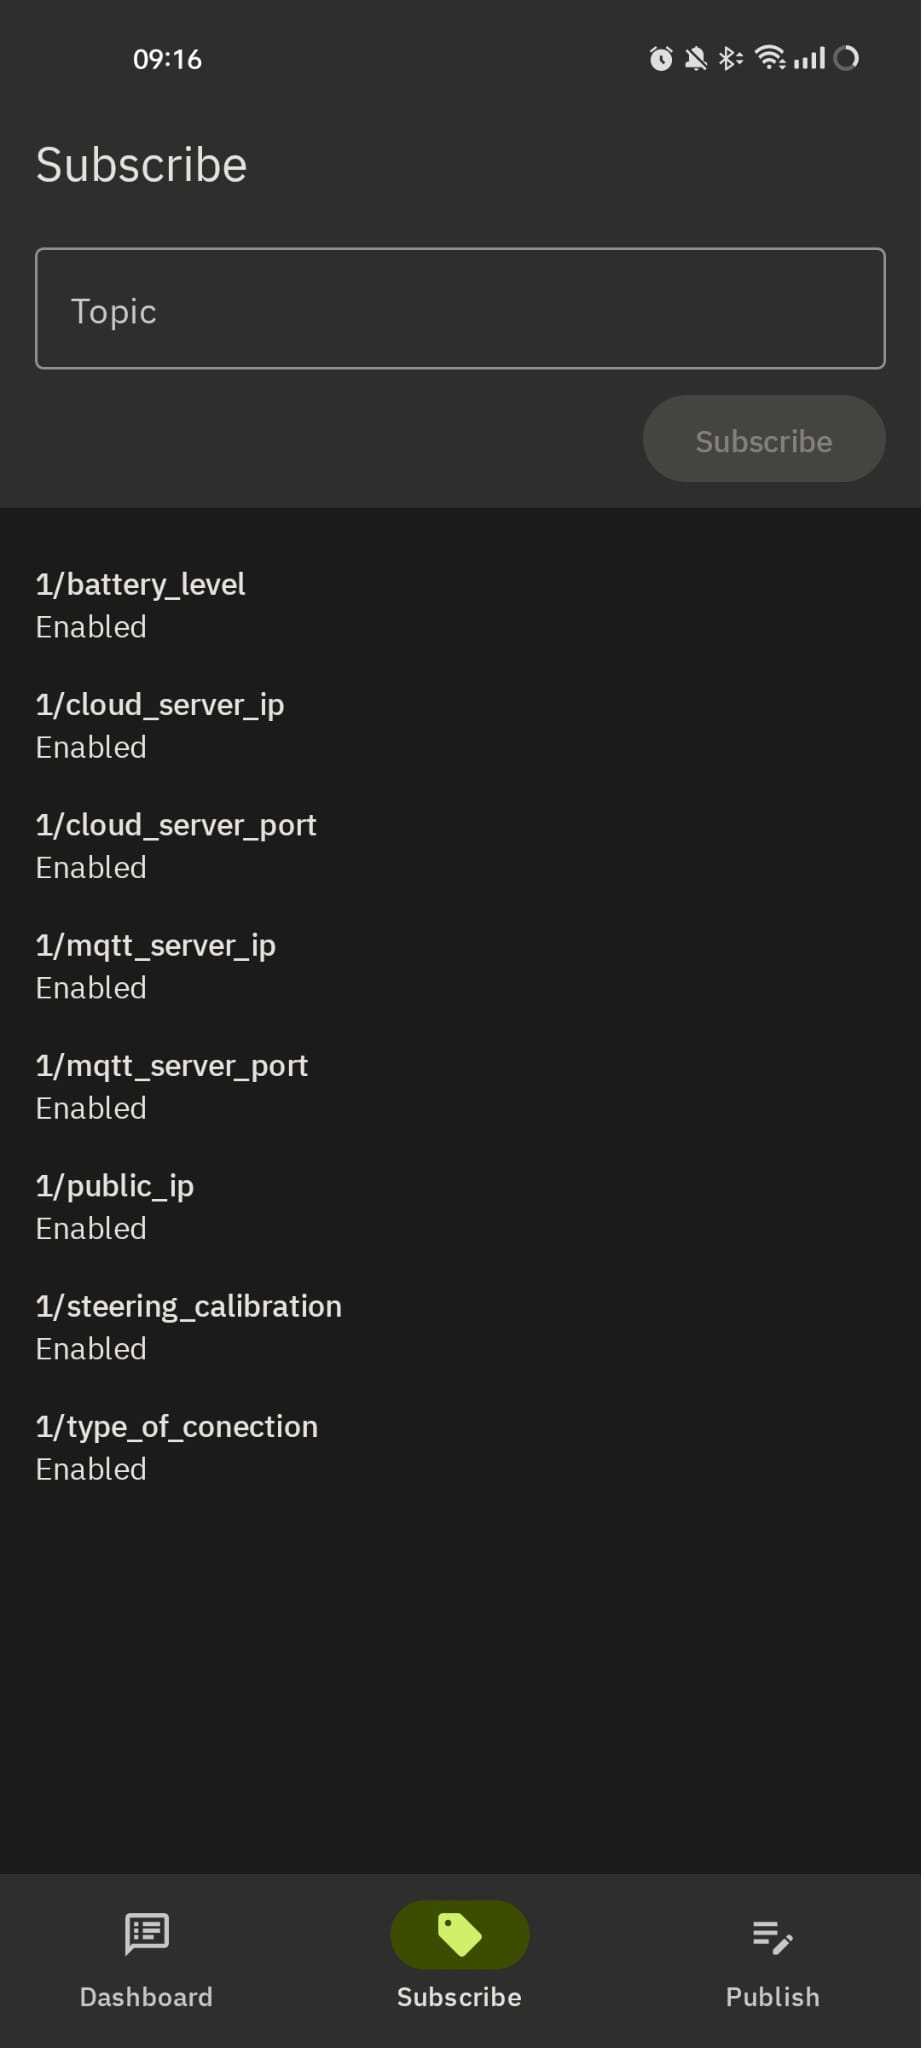
\includegraphics[width=0.4\textwidth]{Imagenes/Rendimiento/mosquitto1.jpeg}}
    \hspace{0.5cm}
    \subfloat[Información mostrada al iniciar la conexión\label{fig:mosq3}]{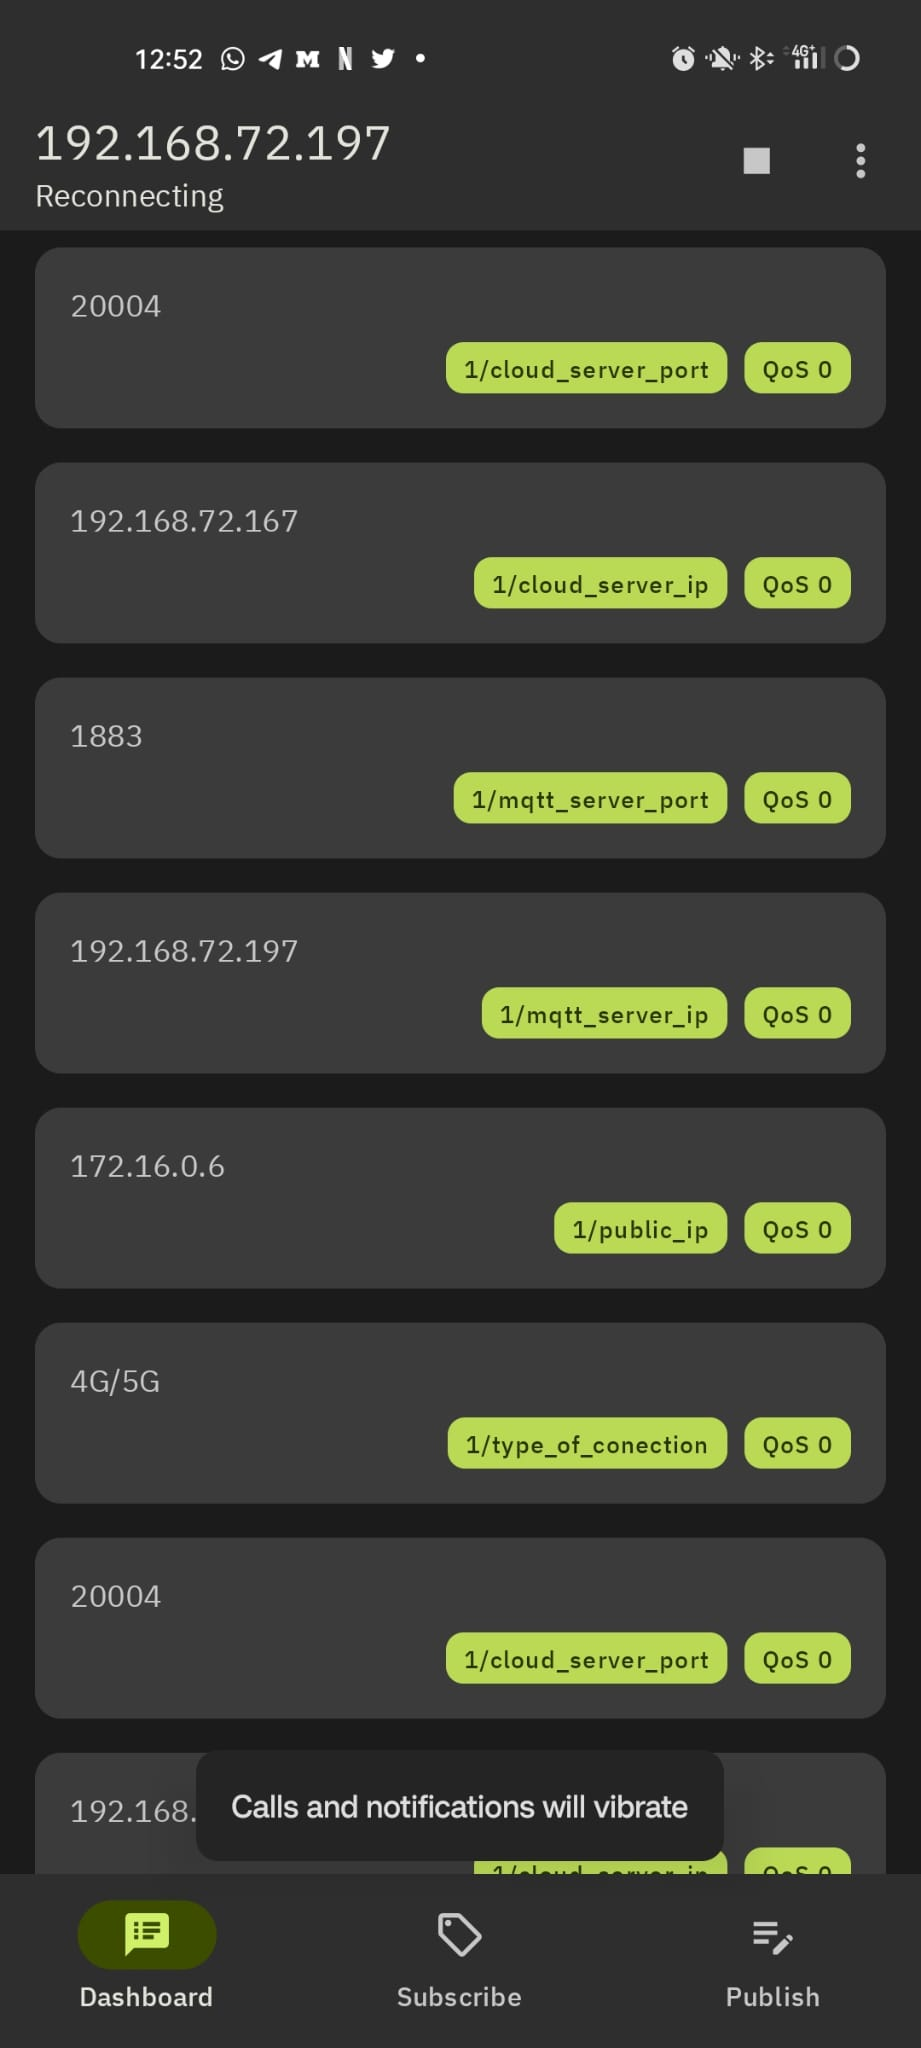
\includegraphics[width=0.4\textwidth]{Imagenes/Rendimiento/mosquitto3.jpeg}}
    \caption{Capturas de pantalla de la aplicación móvil MyMQTT para cliente suscrito}
\end{figure}


\item Tras configurar tanto el servidor como el cliente mosquitto, lanzamos el servicio y comprobamos su estado usando los comandos:
\begin{lstlisting}
	sudo systemctl start mosquitto
	sudo systemctl status mosquitto
\end{lstlisting}


\item Para comunicarnos con el coche, publicaremos los tópicos que se indican en el manual de configuración del coche, como podemos ver en la imagen \ref{mosquitto2}:

 \begin{figure}[H]
    \centering
    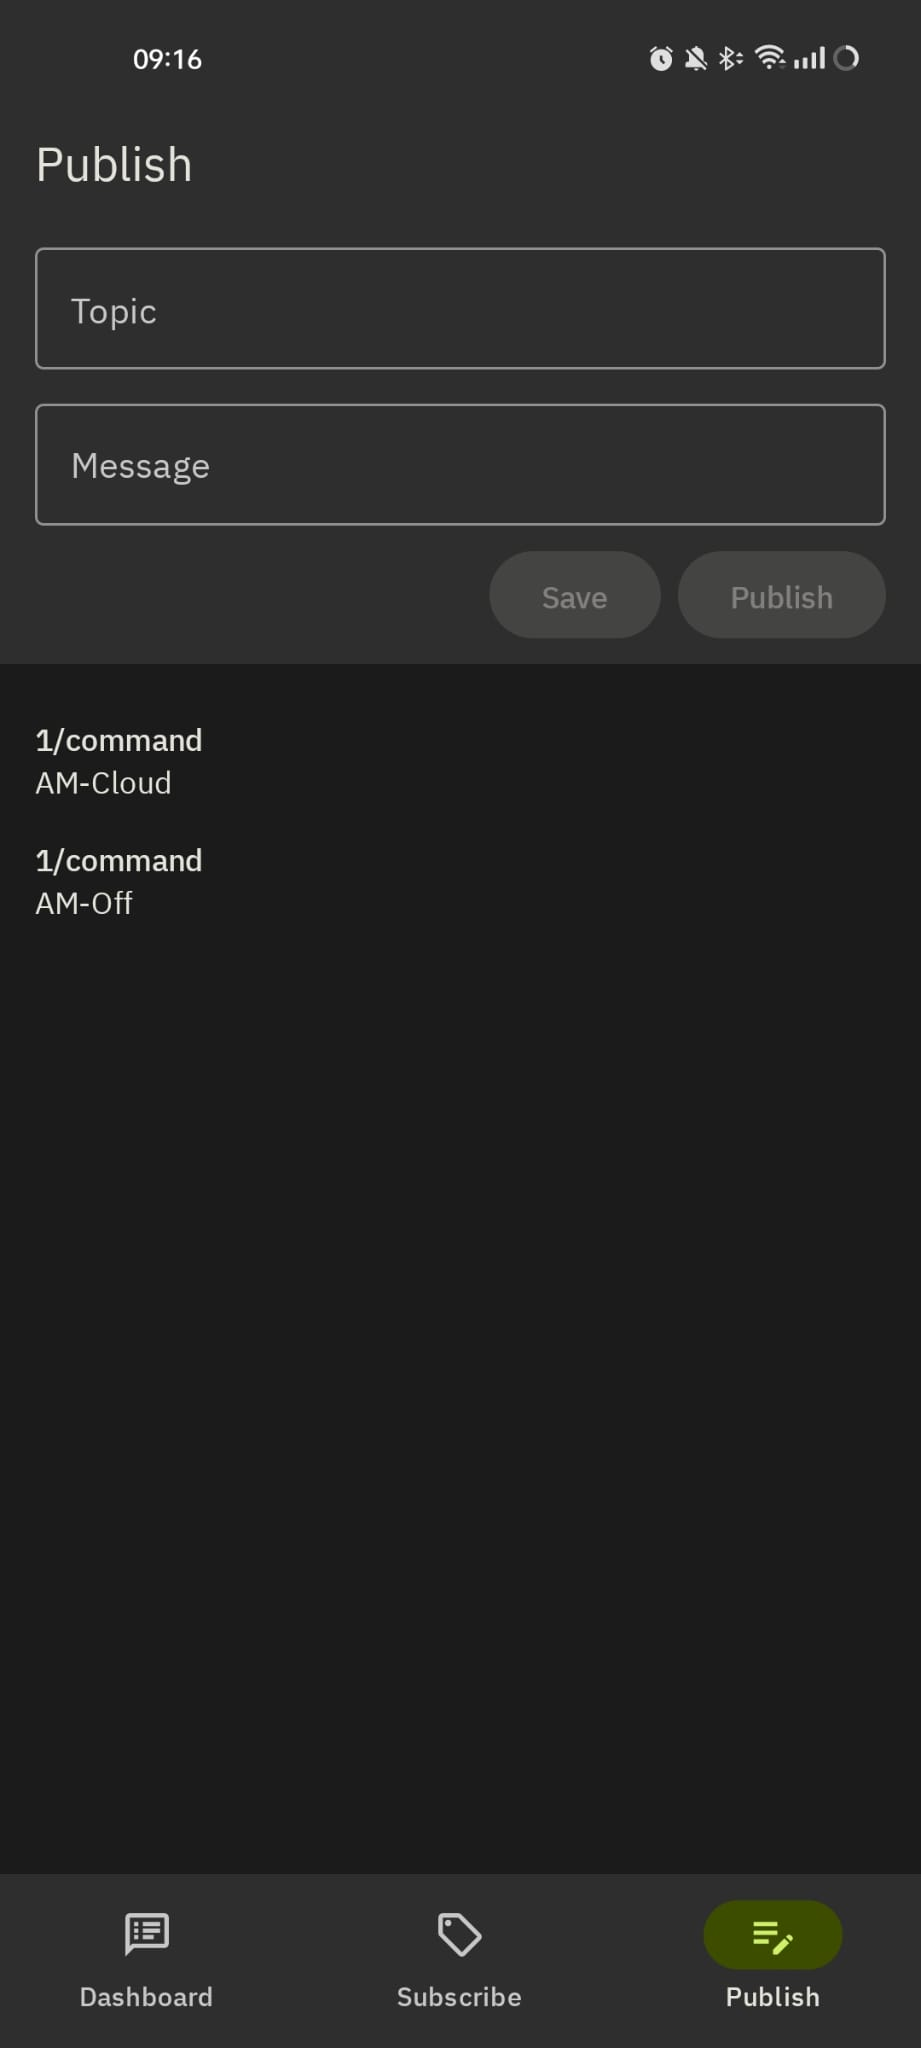
\includegraphics[width=0.35\textwidth]{Imagenes/Rendimiento/mosquitto2.jpeg}
    \caption{Publicación de comandos desde el móvil}
    \label{mosquitto2}
\end{figure}

\end{enumerate}
